% ****** Start of file apssamp.tex ******
%
%   This file is part of the APS files in the REVTeX 4.1 distribution.
%   Version 4.1r of REVTeX, August 2010
%
%   Copyright (c) 2009, 2010 The American Physical Society.
%
%   See the REVTeX 4 README file for restrictions and more information.
%
% TeX'ing this file requires that you have AMS-LaTeX 2.0 installed
% as well as the rest of the prerequisites for REVTeX 4.1
%
% See the REVTeX 4 README file
% It also requires running BibTeX. The commands are as follows:
%
%  1)  latex apssamp.tex
%  2)  bibtex apssamp
%  3)  latex apssamp.tex
%  4)  latex apssamp.tex
%
\documentclass[%
 reprint,
%superscriptaddress,
%groupedaddress,
%unsortedaddress,
%runinaddress,
%frontmatterverbose, 
%preprint,
%showpacs,preprintnumbers,
%nofootinbib,
%nobibnotes,
%bibnotes,
 amsmath,amssymb,
 aps,
%pra,
%prb,
%rmp,
%prstab,
%prstper,
%floatfix,
]{revtex4-1}

\usepackage{graphicx}% Include figure files
\usepackage{dcolumn}% Align table columns on decimal point
\usepackage{bm}% bold math
%\usepackage{hyperref}% add hypertext capabilities
%\usepackage[mathlines]{lineno}% Enable numbering of text and display math
%\linenumbers\relax % Commence numbering lines

%\usepackage[showframe,%Uncomment any one of the following lines to test 
%%scale=0.7, marginratio={1:1, 2:3}, ignoreall,% default settings
%%text={7in,10in},centering,
%%margin=1.5in,
%%total={6.5in,8.75in}, top=1.2in, left=0.9in, includefoot,
%%height=10in,a5paper,hmargin={3cm,0.8in},
%]{geometry}

\begin{document}

\preprint{APS/123-QED}

\title{Homework 5}% Force line breaks with \\

\author{Ho Lun Tang}


\author{Hong Yao}
 
\affiliation{
Department of Physics, Virginia Tech, Blacksburg, VA 24060, USA 
}%



\date{\today}% It is always \today, today,
             %  but any date may be explicitly specified


\maketitle

%\tableofcontents

\section{Linear Chain of Oscillators}

In this section, we consider a system with $N$ particles of mass $m$. The particles can only move in the x-direction(1 dimensional problem). They are each connected to their neighbor by a spring with spring constant $k$. We give the equations of motion of each particles and then find out the recursion relation between the solution of the equations. We also show the normal modes of the system.
\subsection{Equation of Motion}
We consider the coordinate of $q_j$ as the displacement from the equilibrium position of $j$-th particle.

For the $n$-th particle, we have
\begin{equation}
    m\ddot{q}_n=-k(q_n-q_{n-1})+k(q_{n+1}-q_n).
    \label{eom}
\end{equation}
By simplifying it, we got
\begin{equation}
    m\ddot{q}_n=k(q_{n-1}+q_{n+1}-2q_n).
\end{equation}
where $1<n<N$.
From Eq.(\ref{eom}), we can write down the Lagrangian of the system
\begin{equation}
    L=\sum_n\frac{1}{2}\dot{q}_n^2+\sum_n\frac{1}{2}k(q_{n}-q_{n-1})^2.
\end{equation}
\subsection{Recursion Relation between Coefficients of Oscillation Function}
We assume the solution for the Eq.(\ref{eom}) have the following form
\begin{equation}
    q_n(t)=A_ne^{i\Omega t}.
    \label{formoffuntion}
\end{equation}
Take Eq.(\ref{formoffuntion}) into the Equation of Motion Eq.(\ref{eom}), we will get
\begin{equation}
    mA_n\Omega^2e^{i\Omega t}=k(2A_ne^{i\Omega t}-A_{n+1}e^{i\Omega t}-A_{n-1}e^{i\Omega t}).
\end{equation}
By simplifying above equation, we can get the recursion relation between coefficients
\begin{equation}
    (2k-m\Omega^2)A_n=kA_{n-1}+kA_{n+1}.
    \label{recursion}
\end{equation}
\subsection{Normal Modes of the System}
We assume the coefficients $A_n$ have the following form
\begin{equation}
    A_n=A\sin{nq},
\end{equation}
where $A$ is the oscillation amplitude. Take the above Equation into Eq.(\ref{recursion}), we will have
\begin{equation}
    (2k-m\Omega^2)\sin{nq}=k(\sin{(n+1)q}+\sin{(n-1)q}).
\end{equation}
By simplifying it, we finally get
\begin{equation}
    \Omega^2=\frac{4k}{m}\sin^2{\frac{q}{2}}. 
\end{equation}
Since we have $q_0=0=q_{N+1}$, we have the following relation
\begin{equation}
\begin{aligned}
\sin{[0\cdot q]}&=0\\
\sin{[(N+1)\cdot q]}&=0
\end{aligned}.
\label{boundry}
\end{equation}
From Eq.(\ref{boundry}), we can find that
\begin{equation}
    q=\frac{p\cdot\pi}{N+1},
\end{equation}
where $p$ is an arbitrary integer. Finally, we get
\begin{equation}
    \Omega=2\sqrt{\frac{k}{m}}\sin{\frac{p\pi}{2(N+1)}},
\end{equation}
where $p$ is an integer and $p\in[0,4(N+1)]$ .

\section{Precession of the equinoxes}
In this section, we consider the precession of the equinoxes of the Earth. We give the first non-trivial term in the multipole expansion in the potential function and then derive the average potential from the Moon. Then, we give the Lagrangian for the motion and derive the Euler-Lagrange Equation for the motion. Finally we will calculate the period for the precession of the earth due to the effect of the Sun and the Moon.
\subsection{The First Non-trivial Entry in the Multipole Expansion of Potential Function}
We have the multipole expansion of the gravitational potential $V$ of a distribution of $N$ masses $m_i$ in following form
\begin{equation}
    V=-\frac{GM}{r}\sum_{j=0}^{N}m_j(\frac{r'_j}{r})^nP_n(\cos{\psi_j})
\end{equation}
\begin{equation}
\begin{aligned}
    V_1&=-\frac{GM}{r}\sum_{j=0}^{N}m_j\left(\frac{r'_j}{r}\right)P_1(\cos \psi_j) \\
    &=-\frac{GM}{r^2}\sum_{j=0}^{N}m_jr'_j\cos \psi_j
\end{aligned}
\end{equation}
The summation $\sum_{j=0}^{N}m_jr'_j\cos \psi_j$ is the projection of the center of mass on the vector $\vec{r}$, since $r'_j$ and $r$ are measured from the center of mass, the center of mass and hence the projection on $\vec{r}$ are zero.
\begin{equation}
\begin{aligned}
    V_2&=-\frac{GM}{r^3}\sum_{j=0}^{N}m_jr'_j^2\left[\frac{1}{2}\left(3\cos^2\psi_j-1\right)\right] \\
    &=\frac{GM}{2r^3}\sum_{j=0}^{N}m_jr'_j^2\left(3\sin^2\psi_j-2\right) \\
    &=\frac{GM}{2r^3}\left(3I_r-2\sum_{j=0}^{N}m_jr'_j^2\right)
\end{aligned}
\end{equation}
Since $m_j r'_j^2=m_j(x'_j^2+y'_j^2+z'_j^2)=\frac{1}{2}m_j(I_1+I_2+I_3)$,
\begin{equation}
    V_2=\frac{GM}{2r^3}\left[3I_r-\left(I_1+I_2+I_3\right)\right].
\end{equation}
\subsection{The Average Potential for the Earth}
We assume that the shape of the Earth only deviates slightly from sphere and then we only preserve first 2 terms in the potential function
\begin{equation}
    V=-\frac{GMm}{r}+\frac{GM}{2r^3}\left[3I_r-\left(I_1+I_2+I_3\right)\right],
\end{equation}
where $m$ is the mass of the Earth.

For the Earth, we have $I_1=I_2$, thus
\begin{equation}
     V=-\frac{GMm}{r}+\frac{GM}{2r^3}\left[3I_r-\left(2I_1+I_3\right)\right].
     \label{potential}
\end{equation}
We set angle of $\vec{r}$ relative to the principal z axis to be $\gamma$. Then, we have the following relation
\begin{equation}
    I_r=I_1+(I_3-I_1)\cos^2{\gamma}.
\end{equation}
Thus, Eq.(\ref{potential}) becomes
\begin{equation}
    V=-\frac{GMm}{r}+\frac{GM(I_3-I_1)}{2r^3}(3\cos^2{\gamma}-1).
\end{equation}
\begin{figure}
    \centering
    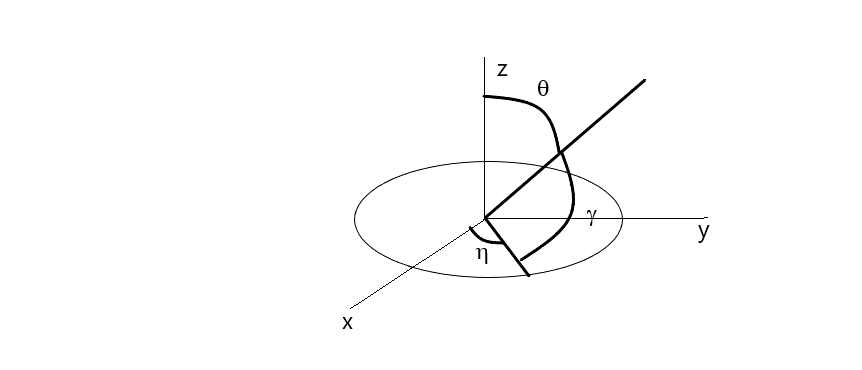
\includegraphics[scale=0.4]{PrincipalCoordinate.png}
    \caption{Angles between principal coordinate and coordinate}
    \label{fig:my_label}
\end{figure}
We consider the angle between the principal z axis and the z axis as $\theta$, and the angle between $\vec{r}$ and x axis as $\eta$, which is showed in Fig.(\ref{fig:my_label}). Since the Moon and the Earth rotate on the same plane, $\vec{r}$ lies on x-y plane. Thus, we have
\begin{equation}
    \cos{\gamma}=\sin{\theta}\cos{\eta}.
\end{equation}
Then the potential becomes
\begin{equation}
     V=-\frac{GMm}{r}+\frac{GM(I_3-I_1)}{2r^3}(3\sin^2\theta\cos^2\eta-1).
\end{equation}

Since the period of precession is much longer than the period of Moon, we can consider $\theta=\rm const$. Thus, the average potential for a period is
\begin{equation}
    \overline{V}=\frac{\int_0^{2\pi}[-\frac{GMm}{r}+\frac{GM(I_3-I_1)}{2r^3}(3\sin^2\theta\cos^2\eta-1)]\mathrm{d}\eta}{\int_0^{2\pi}\mathrm{d}\eta}.
\end{equation}
Finally, we get the average potential for the Earth
\begin{equation}
    \overline{V}=-\frac{GMm}{r}+\frac{GM(I_3-I_1)}{2r^3}(\frac{3}{2}\sin^2\theta-1)
\end{equation}
\subsection{The Average Potential for the Earth}
The Lagrangian is 
\begin{align*}
    L&=T-V \\
    &=\frac{1}{2}I_1\omega_1^2+\frac{1}{2}I_2\omega_2^2+\frac{1}{2}I_3\omega_3^2-\overline{V} \\
    &=\frac{1}{2}I_1\left(\omega_1^2+\omega_2^2\right)+\frac{1}{2}I_3\omega_3^2-\overline{V}
\end{align*}
Using Euler angles,
\begin{align}
    \omega_1&=\dot{\omega}\sin \theta\sin \psi+\dot{\theta}\cos\psi, \\
    \omega_2&=\dot{\phi}\sin\theta\cos\psi-\dot{\theta}\sin\psi, \\
    \omega_3&=\dot{\phi}\cos{\theta}+\dot{\psi},
\end{align}
we can rewrite the Lagrangian as
\begin{equation}
    L=\frac{I_1}{2}(\dot{\theta}^2+\dot{\phi}^2\sin^2\theta)+\frac{I_3}{2}(\dot{\psi}+\dot{\phi}\cos\theta)^2-\overline{V}
\end{equation}
The ELE corresponding to $\theta$ is 
\begin{equation}
    I_1\dot{\phi}^2\sin\theta\cos\theta-I_3\dot{\phi}\sin\theta(\dot{\psi}+\dot{\phi}\cos\theta)-\frac{\partial\overline{V}}{\partial\theta}=I_1\ddot{\theta}
\end{equation}
We assume no nutation,so we take $\ddot{\theta}$=0. We have
\begin{equation}
    \sin\theta\left(I_1\dot{\phi}^2\cos\theta-I_3\dot{\phi}\omega_3+\frac{\partial\overline{V}}{\partial\cos\theta}\right)=0
\end{equation}
Since the precession is much slower than the rotation of the earth, i.e. $\dot{\phi}\ll\omega_3$, we can just omit the $\dot{\phi}^2$ term.
\begin{equation}
\begin{aligned}
    \dot{\phi}&=\frac{1}{I_3\omega_3}\frac{\partial\overline{V}}{\partial\cos\theta} \\
    &=-\frac{3GM}{2\omega_3r^3}\frac{I_3-I_1}{I_3}\cos\theta \\
    &=-\frac{3}{2}\frac{\omega_0^2}{\omega_3}\frac{I_3-I_1}{I_3}\cos\theta,
\end{aligned}
\label{angularvelocity}
\end{equation}
where $\omega_0$ is the orbital frequency of moon or sun respectively.

We have the mass of Moon and Sun that $M_{\mathrm{moon}}\approx7.349\times10^{22}\mathrm{Kg}$ and $M_{\mathrm{sun}}\approx1.9891\times10^{30}\mathrm{Kg}$. And we also have the distance from the Sun or the Moon to the Earth that $r_{\mathrm{moon}}\approx3.843\times10^5\mathrm{Km}$ and $r_{\mathrm{sun}}\approx1.5\times10^8\mathrm{Km}$. Take these quantities into Eq.(\ref{angularvelocity}), we will get \begin{equation}
\begin{aligned}
  \dot{\phi}_{\mathrm{sun}}\approx15.77''/\mathrm{year}  
  \\\dot{\phi}_{\mathrm{moon}}\approx34.54''/\mathrm{year}
\end{aligned}
\end{equation}
Finally, we will find out the precession period due to the Sun and the Moon
\begin{equation}
\begin{aligned}
T_{\mathrm{sun}}\approx81113.76(\mathrm{year})\\
T_{\mathrm{moon}}\approx37035.66(\mathrm{year})
\end{aligned}
\end{equation}

If we want to combine effects from the sun and moon, one way to approximate is to add up the two individual precession,
\begin{equation}
\begin{aligned}
    \dot{\phi}_{tot}&\approx\dot{\phi}_{\mathrm{sun}}+\dot{\phi}_{\mathrm{moon}} \\
    &=50.31''/\mathrm{year},
\end{aligned}
\end{equation}
and the period is 25,760.29 years, about 26,000 years.
\end{document}
%
% ****** End of file apssamp.tex ******